\chapter{Πειραματισμοί και αποτελέσματα}
\label{chapter:experiments}
\section{Το πρόβλημα και η προτεινόμενη λύση}
Οι αλγόριθμοι και τα παραδείγματα που αναφέρθηκαν στο κεφάλαιο \ref{chapter:tl} αφορούσαν αλγόριθμους οι οποίοι δεν είναι πραγματικού χρόνου και εμπεριέχουν μεγάλο πλήθος παραμέτρων και άρα μπορούν να χειριστούν περισσότερα χαρακτηριστικά των πεδίων ορισμού. Αντίθετα, οι αλγόριθμοι πραγματικού χρόνου μπορούν να χειριστούν μικρότερο πλήθος χαρακτηριστικών με αναμενόμενο αποτέλεσμα να δυσχεραίνεται η μεταφερσιμότητά τους.

Επιπλέον, τα νευρωνικά δίκτυα εντοπισμού αντικειμένων χρειάζεται να εντοπίζουν ένα αντικείμενο σε οποιαδήποτε θέση πάνω στην εικόνα. Στα δίκτυα πραγματικού χρόνου υπεύθυνος για τον εντοπισμό ενός αντικειμένου σε μία περιοχή είναι ένας νευρώνας. Αυτό επιταχύνει τον χρόνο εκτέλεσης του δικτύου, ωστόσο κάνει πιο δύσκολη την εκπαίδευση, αφού όλοι σχεδόν οι νευρώνες θα πρέπει να μπορούν να εντοπίσουν κάθε είδους αντικείμενο (που ανήκει στο σύνολο δεδομένων) στην περιοχή για την οποία είναι υπεύθυνοι. Αυτό συντελεί με τη σειρά του σε επιπλέον δυσκολία στη μεταφερσιμότητα κάνοντας τη σχεδόν αδύνατη, στα τελευταία επίπεδα του νευρωνικού.

Δεν υπάρχει κάποια αναφορά (εν γνώσει του συγγραφέα) σε δοκιμές για τη μεταφερσιμότητα των παραμέτρων νευρωνικών δικτύων εντοπισμού αντικειμένων που λειτουργούν σε πραγματικό χρόνο, εκτός από την πολύ πρόσφατη στο \cite{82}. Ωστόσο, σε αυτή την εργασία δε μελετάται με τον ίδιο τρόπο η μεταφερσιμότητα των παραμέτρων. Οπότε, πριν μπορέσει να υπάρξει οποιαδήποτε μελλοντική εφαρμογή θα πρέπει να γίνουν οι πειραματισμοί που παρουσιάζονται παρακάτω.

\section{Το πείραμα}
\label{section:TheExperiment}
Τα πειράματα που απαιτούνται είναι η χρήση ενός νευρωνικού δικτύου εντοπισμού αντικειμένων πραγματικού χρόνου για την πραγματοποίηση πρώτα του πειράματος που περιγράφεται στην ενότητα \ref{section:transferability}. Πρώτα, περιγράφονται τα θεωρητικά βήματα αυτού, μετά η διερεύνηση των αρχικών συνθηκών και τέλος τα αποτελέσματα. Σε μετέπειτα εργασία που περιγράφεται στο κεφάλαιο \ref{chapter:futures} κρίνεται σκόπιμη η υλοποίηση και του πειράματος που περιγράφεται στην ενότητα \ref{section:catastrophicForgetting}, ως μία άλλη σκοπιά στο πρόβλημα.

\subsection{Τα βήματα του πειράματος}
Σε αυτό το πείραμα παρουσιάζεται η συμπεριφορά της απλής επαγωγικής μετάδοσης γνώσης σε νευρωνικά δίκτυα εντοπισμού αντικειμένων πραγματικού χρόνου. Μέσω της συμπεριφοράς αυτής θα γίνει σαφές αν θα πρέπει να προτιμάται η μετάδοση γνώσης ή η μάθηση πολλαπλών έργων στα νευρωνικά δίκτυα εντοπισμού αντικειμένων πραγματικού χρόνου. Η μάθηση πολλαπλών έργων ωστόσο δεν μπορεί να γίνει για έναν οποιοδήποτε αριθμό κλάσεων αντικειμένων, διότι το δίκτυο για ικανά μεγάλο αριθμό μπορεί να σταματήσει να συμπεριφέρεται ως δίκτυο πραγματικού χρόνου.

Επιπρόσθετα, ήδη ο μεγάλος αριθμός κλάσεων δημιουργεί πρόβλημα στο SqueezeDet από άποψη της μνήμης που χρησιμοποιεί. Ο σκοπός δημιουργίας του δικτύου είναι αυτό να έχει μικρή μνήμη, ώστε να μπορεί να χρησιμοποιηθεί από μικρής ισχύος ενσωματωμένες συσκευές. Αν αυξηθεί ο αριθμός των κλάσεων κατά πολύ, το δίκτυο θα παύσει να λειτουργεί σωστά. Ο τύπος του μεγέθους του τελευταίου επιπέδου του SqueezeDet παρουσιάζεται στην παρακάτω εξίσωση:
$$
final\_layer\_shape = 3 \times 3 \times K(C+ 1 + 4)
$$
με $K$ τον αριθμό των υπεύθυνων νευρώνων ανά περιοχή πλέγματος και $C$ τον αριθμό των κλάσεων. Για αυτό το λόγο, όλες οι εκπαιδεύσεις θα πρέπει να περιορίζονται σε μικρό αριθμό κλάσεων.

Για την πραγματοποίηση του πειράματος επιλέχθηκαν τα σύνολα δεδομένων PASCAL\_VOC και KITTI. Αρχικά στο πείραμα χωρίζονται δύο σύνολα δεδομένων, ονόματι A, B, διαλέγοντας το KITTI ως το (Α) και το υποσύνολο του PASCAL\_VOC που εμπεριέχει τρεις (ιδανικά τυχαίες) κλάσεις (Β).

Τα βήματα που ακολουθούνται για την πραγματοποίηση του πειράματος είναι τα εξής:
\begin{enumerate}
\item Εκπαίδευση ολόκληρου του SqueezeDet στο υποσύνολο δεδομένων Α. Με το πέρας αυτής της εκπαίδευσης το στιγμιότυπο του δικτύου θα ονομάζεται δίκτυο A.
\item Εκπαίδευση ολόκληρου του SqueezeDet στο υποσύνολο δεδομένων B. Με το πέρας αυτής της εκπαίδευσης το στιγμιότυπο του δικτύου θα ονομάζεται δίκτυο B.

\item{Σε ένα καινούριο δίκτυο τύπου SqueezeDet αντιγράφονται τα $n$ πρώτα επίπεδα του δικτύου B σε αυτό και τα υπόλοιπα αρχικοποιούνται τυχαία με τη μέθοδο Xavier. Το δίκτυο εκπαιδεύεται στο σύνολο δεδομένων B. Τα $n$ πρώτα επίπεδα του δικτύου παραμένουν σταθερά. Με το πέρας αυτής της εκπαίδευσης το στιγμιότυπο του δικτύου θα ονομάζεται δίκτυο $BnB$.}

\item{Σε ένα καινούριο δίκτυο τύπου SqueezeDet αντιγράφονται τα $n$ πρώτα επίπεδα του δικτύου B σε αυτό και τα υπόλοιπα αρχικοποιούνται τυχαία με τη μέθοδο Xavier. Το δίκτυο εκπαιδεύεται στο σύνολο δεδομένων B. Τα $n$ πρώτα επίπεδα του δικτύου δεν παραμένουν σταθερά και εκπαιδεύονται μαζί με τα υπόλοιπα. Με το πέρας αυτής της εκπαίδευσης το στιγμιότυπο του δικτύου θα ονομάζεται δίκτυο $BnB^+$.}

\item{Σε ένα καινούριο δίκτυο τύπου SqueezeDet αντιγράφονται τα $n$ πρώτα επίπεδα του δικτύου A σε αυτό και τα υπόλοιπα αρχικοποιούνται τυχαία με τη μέθοδο Xavier \cite{77}. Το δίκτυο εκπαιδεύεται στο σύνολο δεδομένων B. Τα $n$ πρώτα επίπεδα του δικτύου παραμένουν σταθερά. Με το πέρας αυτής της εκπαίδευσης το στιγμιότυπο του δικτύου θα ονομάζεται δίκτυο $AnB$.}

\item{Σε ένα καινούριο δίκτυο τύπου SqueezeDet αντιγράφονται τα $n$ πρώτα επίπεδα του δικτύου A σε αυτό και τα υπόλοιπα αρχικοποιούνται τυχαία με τη μέθοδο Xavier. Το δίκτυο εκπαιδεύεται στο σύνολο δεδομένων B. Τα $n$ πρώτα επίπεδα του δικτύου δεν παραμένουν σταθερά και εκπαιδεύονται μαζί με τα υπόλοιπα. Με το πέρας αυτής της εκπαίδευσης το στιγμιότυπο του δικτύου θα ονομάζεται δίκτυο $AnB^+$.}

\end{enumerate}

Τα βήματα 3 έως 6 επαναλαμβάνονται για $n = 1,\hdots,11$ και για τρεις τυχαίους χωρισμούς του συνόλου δεδομένων σε υποσύνολα A, B. Η διαφορά μεταξύ των τεσσάρων εκπαιδεύσεων, παρουσιάζεται καλύτερα στο Σχήμα \ref{fig:tl_exp_config}, το οποίο περιγράφεται και στο \cite{55}. Η κάθε εκπαίδευση γίνεται με συμπερίληψη της μετρικής mAP όπως αναφέρεται στην ενότητα \ref{section:transferability}.


\begin{figure}
\centering
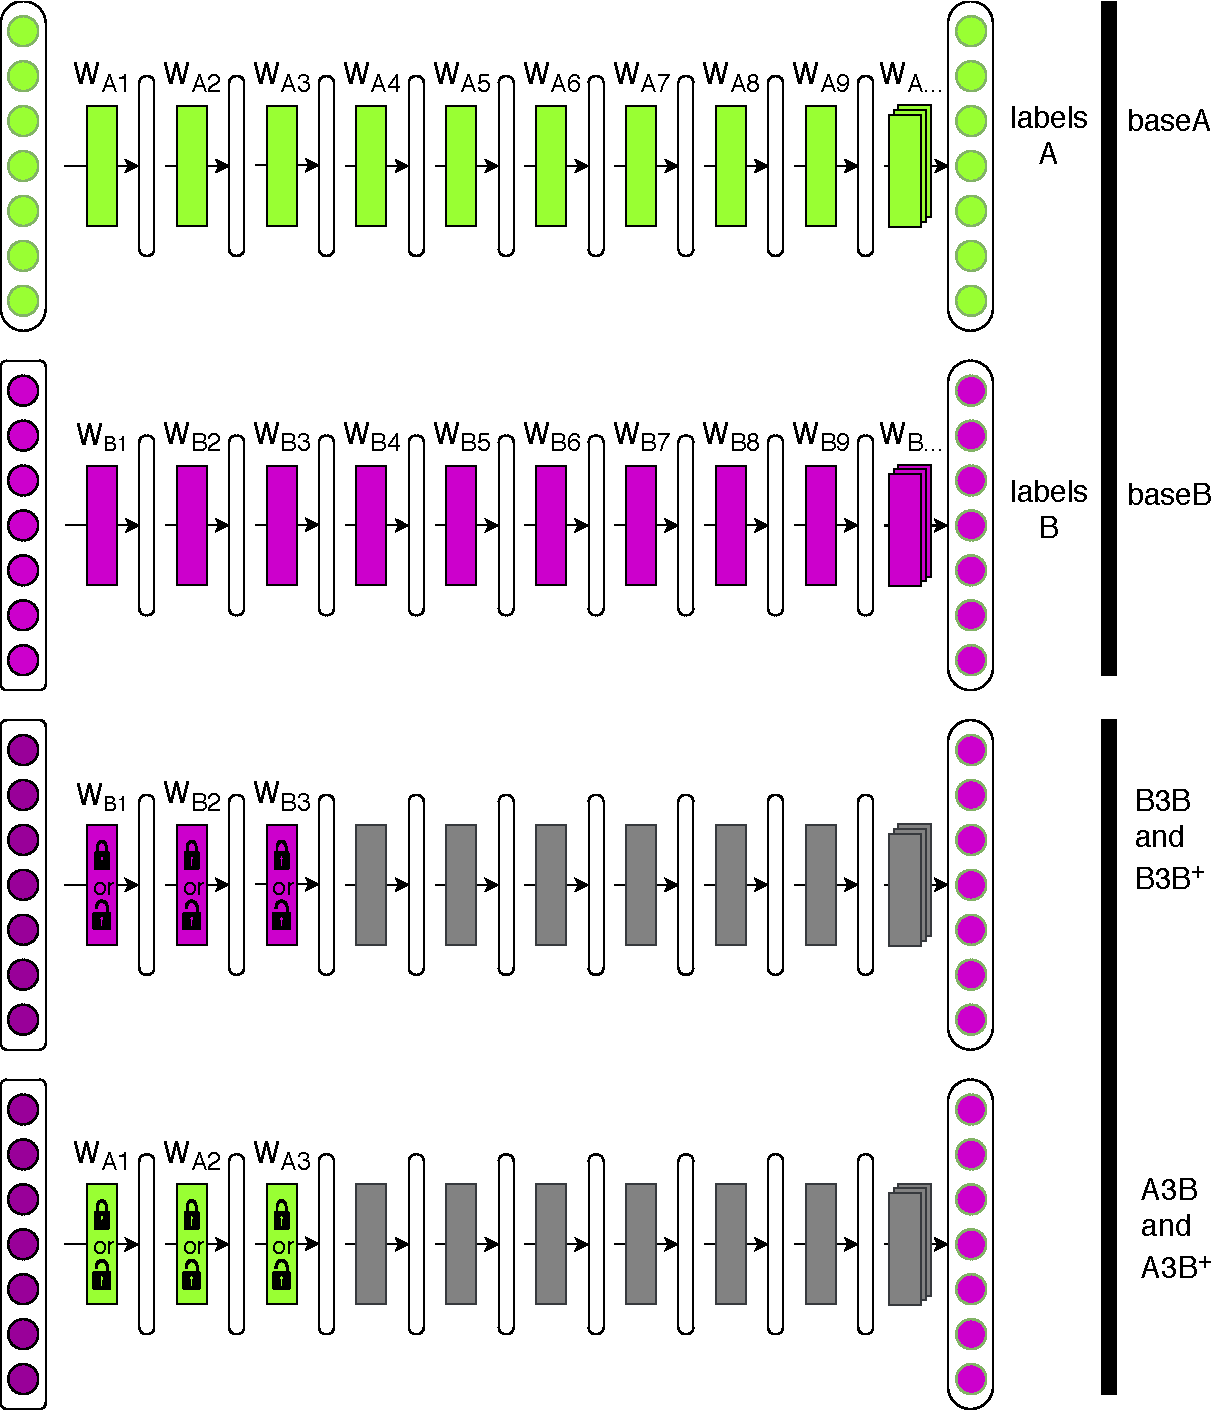
\includegraphics[width = \textwidth]{figures/experiments/tl_exp_config.pdf}
\caption[Οι τέσσερις διαφορετικές αρχικοποιήσεις του δικτύου]{Οι τέσσερις διαφορετικές αρχικοποιήσεις του δικτύου SqueezeDet κατά το πείραμα. Το \textcolor{myGreen}{πράσινο} χρώμα αναφέρεται στα δεδομένα που ανήκουν στο υποσύνολο δεδομένων A όπως και στο δίκτυο A. Ενώ το \textcolor{magenta}{μωβ} χρώμα αναφέρεται στα δεδομένα που ανήκουν στο υποσύνολο δεδομένων B και στο δίκτυο B. Τα ορθογώνια με \textcolor{myGrey}{γκρι} χρώμα δείχνουν τα επίπεδα στα οποία οι παράμετροί τους αρχικοποιούνται με τυχαίες τιμές χρησιμοποιώντας τη μέθοδο Xavier.}
\label{fig:tl_exp_config}
\end{figure}

\subsection{Εκπαίδευση στο σύνολο δεδομένων A}
\label{subsection:Atrain}
Ως σύνολο δεδομένων Α ελήφθη το σύνολο δεδομένων του KITTI, το οποίο είναι αρκετά μεγάλο και είχε σίγουρα ικανοποιητικά αποτελέσματα για το SqueezeDet. Οι κλάσεις στις οποίες εκπαιδεύτηκε το δίκτυο είναι οι "car", "pedestrian", "cyclist" όπως και στην αρχική εργασία. Η διαφορά στο μέγεθος των εικόνων των δύο συνόλων δεδομένων θα οδηγήσει στην ανικανότητα μελέτης του τελευταίου επιπέδου του νευρωνικού ως προς τη μετάδοση γνώσης. Ωστόσο, το τελευταίο επίπεδο θεωρείται σύμφωνα με το αρχικό πείραμα ότι θα δώσει υπερβολικά χαμηλής απόδοσης αποτελέσματα για τα $AnB$ και $AnB^+$. Επιπλέον, δεν μπορεί να γίνει κάποια σύγκριση αν ο παραπάνω αριθμός $n$ είναι ίσος με όλα τα επίπεδα του νευρωνικού, διότι πρόκειται για εκφυλισμένη περίπτωση.

Η εκπαίδευση έγινε στο KITTI για $35000$ επαναλήψεις δίνοντας τα αποτελέσματα που διακρίνονται στο Σχήμα \ref{fig:Atrain}. Η εκπαίδευση δεν προχώρησε σε παραπάνω βήματα, διότι αυτό θα σήμαινε υπέρ-προσαρμογή του δικτύου στο σύνολο δεδομένων του KITTI.

\begin{figure}
\centering
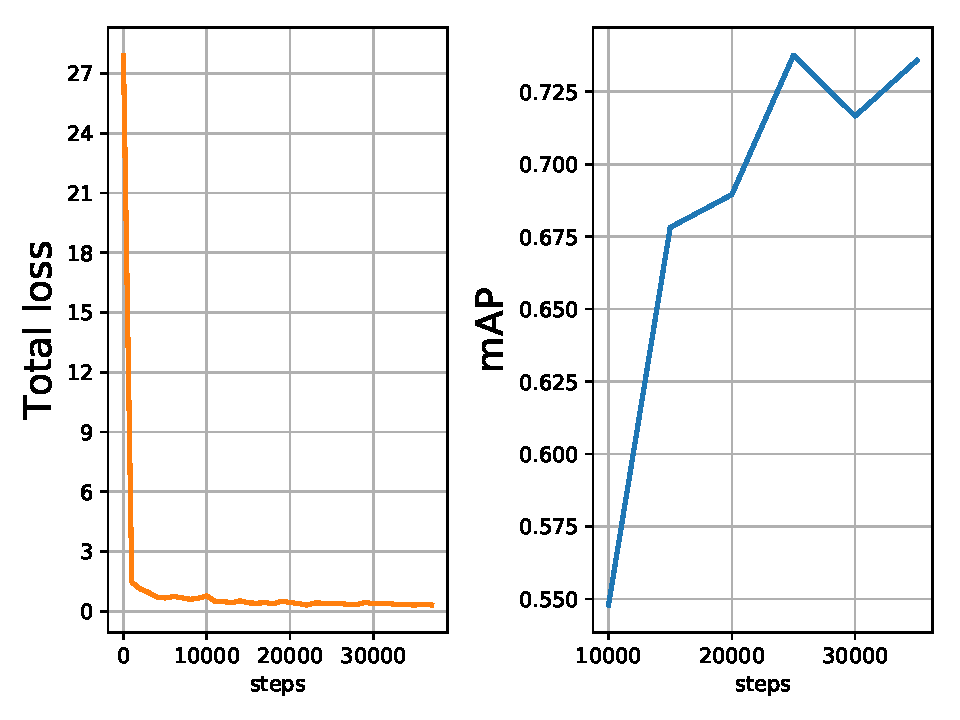
\includegraphics[width = \textwidth]{figures/experiments/Atrain.pdf}
\caption[Η εκπαίδευση του SqueezeDet στο σύνολο δεδομένων A, με χρήση βαρών του ImageNet]{Η εκπαίδευση του SqueezeDet στο σύνολο δεδομένων A (KITTI) με χρήση βαρών του ImageNet. Η χρήση μετάδοσης γνώσης παραμέτρων σε αυτή την εκπαίδευση δεν έχει καμία επιρροή στο πείραμα. Το μέγιστο mAP το οποίο μπορεί να επιτευχθεί δε φαίνεται σε αυτή την εκπαίδευση καθότι θα έπρεπε τα βήματα να είναι ακόμα $15000$ το οποίο μπορεί να οδηγήσει και σε υπέρ-προσαρμογή.}
\label{fig:Atrain}
\end{figure}

\subsection{Εκπαίδευση στο σύνολο δεδομένων Β}
\label{subsection:Btrain}
Το σύνολο δεδομένων Β προέρχεται από το σύνολο δεδομένων PASCAL\_VOC. Η συνολική εκπαίδευση στο συνολικό σύνολο δεδομένων φάνηκε αδύνατη ως επιλογή διότι το SqueezeDet δεν είναι υλοποιημένο με το σκεπτικό να αναγνωρίζει ένα μεγάλο σύνολο δεδομένων, άλλωστε αυτό έδειξαν και τα πειράματα κατά τη συνολική εκπαίδευση του δικτύου σε αυτό το σύνολο δεδομένων όπως φαίνεται και στο Σχήματα \ref{fig:Btrain1}, \ref{fig:Btrain2}. Οπότε, για την εύρεση των υπερπαραμέτρων και του βέλτιστου υποσυνόλου χρειάστηκε να γίνουν αρκετές δοκιμές επιλογής τους. Το σύνολο που επιλέχθηκε ως B ήταν το σύνολο που έχει ως κλάσεις τις "bicycle", "bus", "dog", στο οποίο μετά από εκπαίδευση το δίκτυο επιτυγχάνει mAP $40\%$. Μάλιστα, μετά τις $20000$ επαναλήψεις λάμβανε χώρα το φαινόμενο της υπέρ-προσαρμογής, οπότε και προτείνεται στο συνολικό πείραμα ο πειραματισμός με μόνο $30000$ επαναλήψεις ανά επί μέρους επανεκπαίδευση.

Προκειμένου να επιταχυνθούν οι δοκιμές μεταφέρθηκαν οι παράμετροι του squeezeNet από προηγούμενη εκπαίδευση του στο ImageNet. Αρχικά, επιλέχθηκε ένα τυχαίο σύνολο με κλάσεις τις "aeroplane", "bicycle", "bird" και δοκιμάστηκε η εύρεση τυχαίων υπερπαραμέτρων. Οι μετρήσεις σε αυτό το πρώτο υποσύνολο δεν ήταν καθόλου ικανοποιητικές, καθότι στην καλύτερη περίπτωση το mAP στο σύνολο δεδομένων ελέγχου ήταν $24\%$. Στη συνέχεια έγιναν δοκιμές και σε άλλα τυχαία επιλεγμένα σύνολο οι οποίες φαίνονται στον Πίνακα \ref{table:subsetSearch}. Όλες οι μετρήσεις αφορούν τις πρώτες $45000$ επαναλήψεις κάθε εκπαίδευσης. Δοκιμάστηκε η εκπαίδευση με τη μέθοδο Adam \cite{19}, ωστόσο αυτή είχε ακόμα χειρότερη γενίκευση ($mAP=0.001$) από ότι η μέθοδος Momentum \cite{81} που χρησιμοποιείται από την αρχική έκδοση του SqueezeDet.

\begin{figure}
\centering
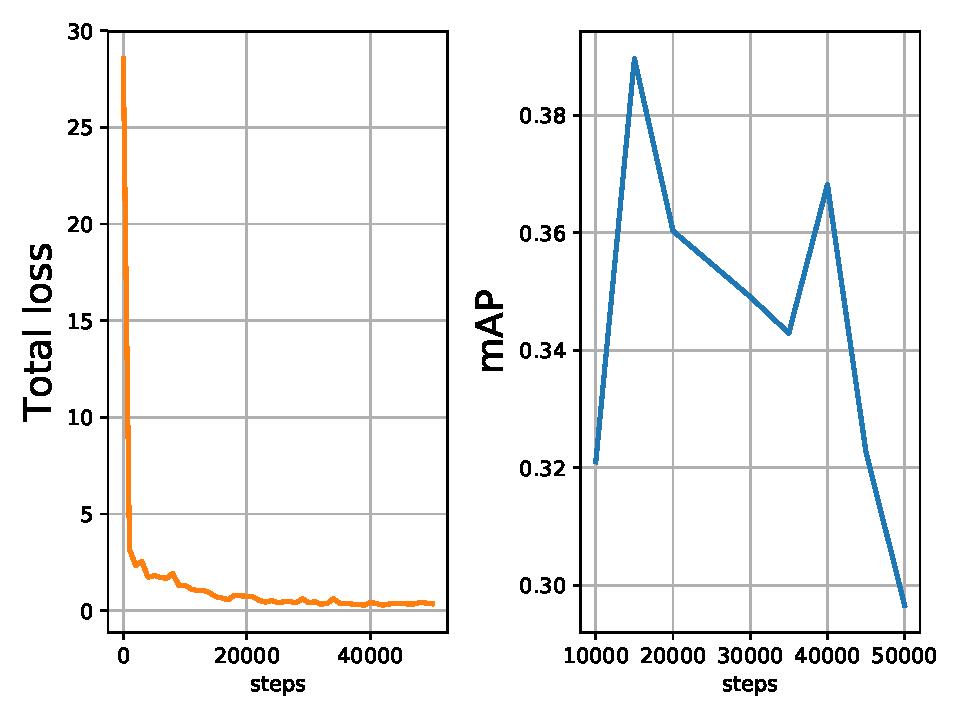
\includegraphics[width = \textwidth]{figures/experiments/Btrain1.pdf}
\caption[Η εκπαίδευση του SqueezeDet στο σύνολο δεδομένων B, με χρήση βαρών του ImageNet]{Η εκπαίδευση του SqueezeDet στο σύνολο δεδομένων B με χρήση βαρών του ImageNet. Η χρήση των βαρών του ImageNet στα επίπεδα του SqueezeDet δείχνει την αρκετά καλύτερη συμπεριφορά την οποία θα μπορούσε να έχει το δίκτυο αν ιδανικά εκπαιδευόταν για πάνω από χίλιες εποχές και σε περισσότερα δεδομένα.}
\label{fig:Btrain1}
\end{figure}

\begin{figure}
\centering
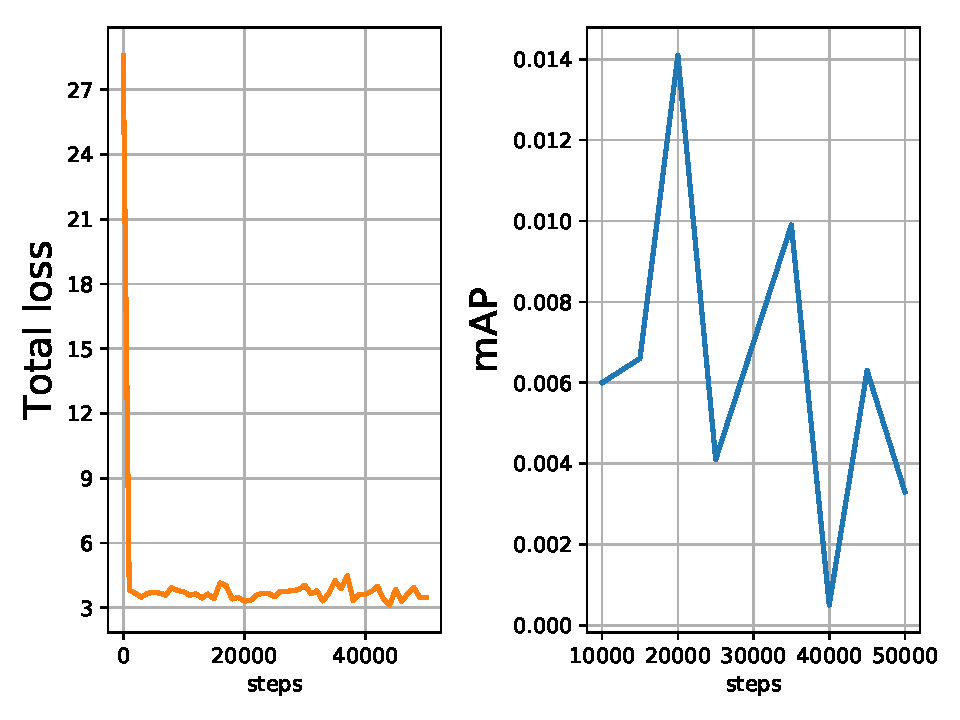
\includegraphics[width = \textwidth]{figures/experiments/Btrain2.pdf}
\caption[Η εκπαίδευση του SqueezeDet στο σύνολο δεδομένων B, χωρίς τη χρήση βαρών του ImageNet]{Η εκπαίδευση του SqueezeDet στο σύνολο δεδομένων B χωρίς τη χρήση βαρών του ImageNet. Η εκπαίδευση κατά αυτό τον τρόπο προφανώς δεν μπορεί να τελειώσει εντός $40000$ επαναλήψεων και θα χρειαστεί μέρες για να φτάσει στο ίδιο αποτέλεσμα. Επίσης, απαιτούνται περισσότερα δεδομένα (όπως παρουσιάζεται παρακάτω) για την επίτευξη ικανοποιητικού mAP. Αυτά όλα βέβαια με την προϋπόθεση πως η εντελώς τυχαία επιλογή παραμέτρων δεν αποκλείει την προσβασιμότητα στις ιδανικές παραμέτρους.}
\label{fig:Btrain2}
\end{figure}

\begin{table}[]
\centering
\caption{Εκπαιδεύσεις σε τυχαία επιλεγμένα υποσύνολα του PASCAL\_VOC.}
\label{table:subsetSearch}
\begin{tabular}{|l|l|}
\hline
\textbf{Υποσύνολο} & βέλτιστο \textbf{mAP} \\ \hline
"aeroplane", "bicycle", "bird" & $24\%$ \\ \hline
"bicycle", "bus", "car" &  $35\%$\\ \hline
"cat", "dog", "bird" & $24\%$  \\ \hline
"cat", "dog", "person" & $34\%$ \\ \hline
"cat", "dog", "bicycle" & $21\%$ \\ \hline
"bicycle", "bus", "dog" & $40\%$ \\ \hline
\end{tabular}
\end{table}
Ένας από τους λόγους για τους οποίους οι εκπαιδεύσεις δεν αποδίδουν υψηλή μετρική mAP είναι ότι οι εικόνες που εισάγονται στο νευρωνικό κατά το πλείστον δεν εμπεριέχουν όλες τις κλάσεις ή πάνω από μία κλάση αντικειμένων.

Τέλος, για να συμπληρωθεί η επιλογή των υπερπαραμέτρων, το μέγεθος της εικόνας που εισάγεται στο πρώτο επίπεδο του δικτύου είναι $(h,w) = (334, 500)$. Η επιλογή αυτή έγινε μετά από στατιστική ανάλυση του συνόλου δεδομένων και βρέθηκε πως ο μέσος όρος των μεγεθών των εικόνων βρισκόταν σε αυτό το σημείο. Επίσης, δοκιμάστηκαν τιμές αρκετά μεγαλύτερες αλλά και σε γειτονικά σημεία και βρέθηκε ότι αυτό το μέγεθος εικόνας δίνει το καλύτερο δυνατό mAP.

\subsection{Τελικά αποτελέσματα}
\label{section:grantExpRes}
Τα τελικά αποτελέσματα του πειράματος φαίνονται στο Σχήμα \ref{fig:grantExpRes} και με λογαριθμικό σκέλος της μετρικής mAP στο Σχήμα \ref{fig:grantExpResLog}. Με μία πρώτη ματιά το πείραμα φαίνεται να μην πέτυχε ως προς τη μεταφερσιμότητα των παραμέτρων. Λόγω αυτού, εξετάστηκε το ενδεχόμενο ο αριθμός των επαναλήψεων να ήταν πολύ μικρός. Οπότε, έγινε επανάληψη των πειραμάτων του δικτύου $AnB^+$ χρησιμοποιώντας $100000$ επαναλήψεις, δηλαδή περίπου $1800$ εποχές.

Η καινούρια επανάληψη των πειραμάτων του $AnB^+$ έδειξε πως η μετρική mAP δεν μπορούσε να βελτιωθεί με τη χρήση περισσότερων εποχών. Οπότε, συνεπάγεται ότι και τα τελικά αποτελέσματα του $AnB$ είναι σωστά, αφού αυτά θα έπρεπε να είναι το πολύ όσο οι τιμές των $AnB^+$. Επίσης, τα αποτελέσματα $BnB, BnB^+$ δοκιμάστηκαν ως προς τις $65000$ επαναλήψεις στα σημεία $n=4$ και $n=5$ δίνοντας ξανά τα ίδια αποτελέσματα. Άρα και οι επανεκπαιδεύσεις των δικτύων $BnB, BnB^+$ δεν απαιτούν παραπάνω επαναλήψεις για να πετύχουν καλύτερη μετρική mAP στο σύνολο ελέγχου. 

Επομένως, κύριο πρόβλημα δεν είναι ο μικρός αριθμός των επαναλήψεων, αλλά μάλλον ο μικρός αριθμός παραδειγμάτων για τη μετεκπαίδευση του δικτύου στο σύνολο Β. Ο μικρός αυτός αριθμός οδηγεί ταυτόχρονα και στην ανικανότητα εκπαίδευσης του δικτύου όπως στην παράγραφο \ref{subsection:Btrain} χωρίς τη μεταφορά παραμέτρων από το ImageNet. Οπότε, η μετεκπαίδευση αυτή παρουσιάζει ένα παράδειγμα στο οποίο οι παράμετροι της εκπαίδευσης του SqueezeNet, που αποτελεί τον κύριο κορμό του SqueezeDet, εκπαιδευμένες στο ImageNet είναι πιο γενικές από τις οποιεσδήποτε παραμέτρους του SqueezeDet μετά από εκπαίδευση του στον εντοπισμό αντικειμένων ενός συνόλου δεδομένων, διότι σε αυτό το σύνολο χρειάζεται οι παράμετροι του SqueezeDet να προσαρμοστούν παραπάνω για τον εντοπισμό συγκεκριμένων αντικειμένων.

Γνωρίζοντας ότι η μετεκπαίδευση δεν εξαρτάται από επιπλέον επαναλήψεις και με κάθε επιφύλαξη ότι στο σύνολο δεδομένων B μπορεί να γίνει εκπαίδευση όπως αυτή δοκιμάστηκε στην παράγραφο \ref{subsection:Btrain}, μπορεί να εξηγηθεί η συμπεριφορά του Σχήματος \ref{fig:grantExpRes} και του Σχήματος \ref{fig:grantExpResLog}. Στο σύνολο που επιλέχθηκε, το δίκτυο παρουσιάζει αρκετά εύθραυστη συν-προσαρμογή για αυτό και τα $7$ πρώτα επίπεδα θα πρέπει να είναι εκπαιδεύσιμα ώστε να μπορέσει να γίνει καλύτερη μετεκπαίδευση και να λειτουργήσει η μεταφορά των παραμέτρων. Επίσης, σε αυτό το σημείο δε βοηθάει ιδιαίτερα η τελειοποίηση (\textit{fine tuning}) καθότι έχει σχεδόν τα ίδια αποτελέσματα. Μάλιστα, αυτά είναι λίγο χειρότερα για τα πρώτα επίπεδα όπως παρουσιάζεται στο Σχήμα \ref{fig:grantExpResLog}. 

Αν τα αποτελέσματα των μετεκπαιδεύσεων των δικτύων $BnB^+$ ήταν καλύτερα από τα $BnB$, τότε θα υπήρχε λόγος σημαντικής βελτίωσης των αποτελεσμάτων στα δίκτυα $AnB^+$ από ότι στα $AnB$. Ωστόσο, τα πειράματα δείχνουν το αντίθετο που σημαίνει ότι η τελειοποίηση (\textit{fine tuning}) δεν πετυχαίνει τίποτα παραπάνω. Βέβαια, εξαιρούνται οι περιπτώσεις για $n \geq 7$, στις οποίες όμως η συμπεριφορά βελτιώνεται το πολύ κατά $1\%$. Για τη μετεκπαίδευση αυτό σημαίνει ότι ακόμα και η καλύτερη περίπτωσή μετάδοσης γνώσης με τελειοποίηση αποτυχαίνει να ανακτήσει υψηλότερη μετρική mAP στο σύνολο ελέγχου.

Όσον αφορά τα δίκτυα $BnB$, οι επανεκπαιδεύσεις των δικτύων αυτών έχουν χειρότερη μετρική mAP στο σύνολο ελέγχου σε όλες τις περιπτώσεις. Η εξήγηση είναι ότι πέρα από ότι το δίκτυο έχει πολλά εύθραυστα επίπεδα στην συν-προσαρμογή, γίνεται επανεκπαίδευση στο ίδιο σύνολο για περισσότερες επαναλήψεις από ότι στην αρχική εκπαίδευση στο σύνολο B. Αυτό σημαίνει ότι το δίκτυο υπέρ-προσαρμόζεται στο σύνολο εκπαίδευσης. Το αποτέλεσμα της υπερ-προσαρμογής είναι να έχει μικρότερη δυνατότητα γενίκευσης στο σύνολο ελέγχου.

\begin{figure}
\centering
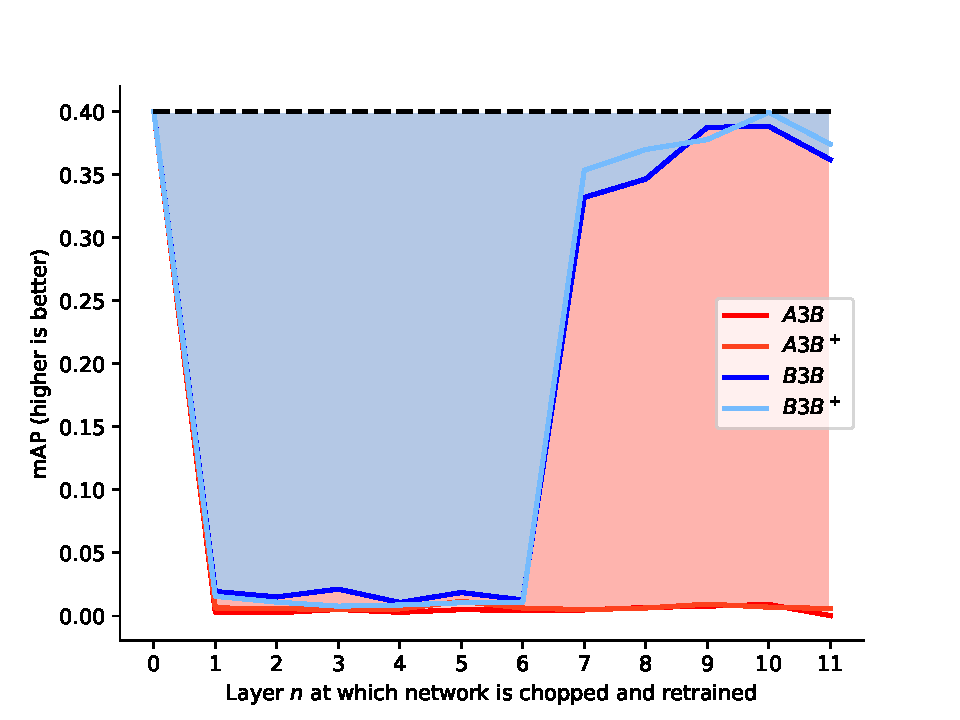
\includegraphics[width=\textwidth]{figures/experiments/grantExp.pdf}
\caption[Η μεταφερσιμότητα των παραμέτρων του SqueezeDet από το σύνολο Α στο σύνολο Β]{Η μεταφερσιμότητα των παραμέτρων του SqueezeDet από το σύνολο Α στο σύνολο Β. Η έντονη μπλε γραμμή είναι το mAP του δικτύου $BnB$, η λιγότερο έντονη του δικτύου $BnB^+$, η έντονα κόκκινη του δικτύου $AnB$ και η λιγότερο έντονη του $AnB^+$.}
\label{fig:grantExpRes}
\end{figure}

\begin{figure}
\centering
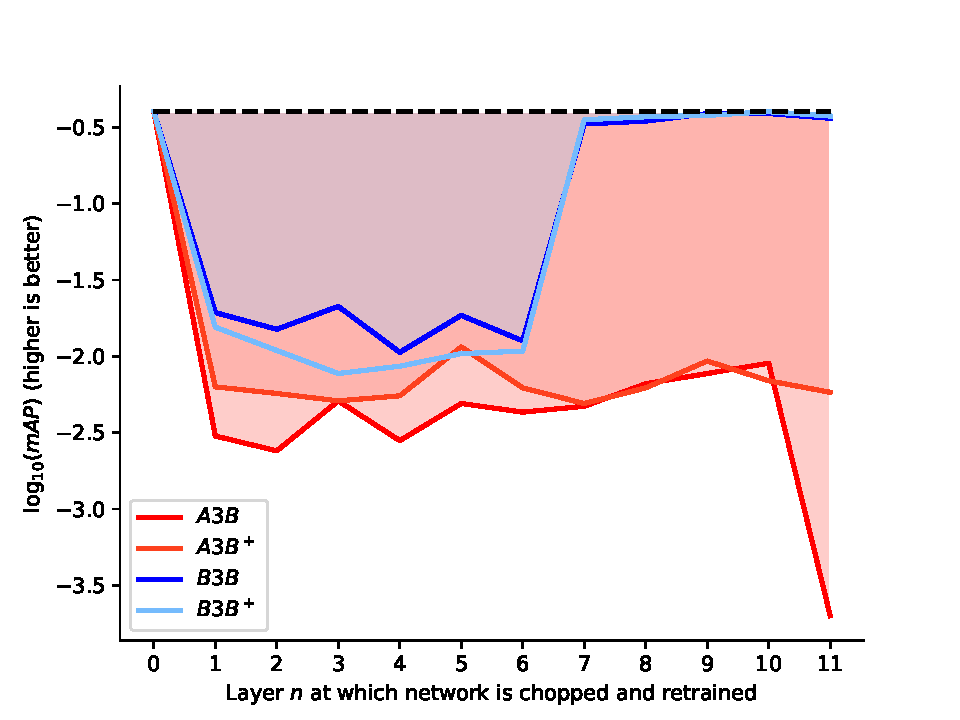
\includegraphics[width=\textwidth]{figures/experiments/grantExpLog.pdf}
\caption[Η μεταφερσιμότητα των παραμέτρων του SqueezeDet από το σύνολο Α στο σύνολο Β σε λογαριθμικό σκέλος]{Η μεταφερσιμότητα των παραμέτρων του SqueezeDet από το σύνολο Α στο σύνολο Β σε λογαριθμικό σκέλος. Η έντονη μπλε γραμμή είναι το mAP του δικτύου $BnB$, η λιγότερο έντονη του δικτύου $BnB^+$, η έντονα κόκκινη του δικτύου $AnB$ και η λιγότερο έντονη του $AnB^+$. Οι διαφορές μεταξύ των $BnB$ και $BnB^+$ διακρίνονται περισσότερο. }
\label{fig:grantExpResLog}
\end{figure}


\section{Αυτόματη επιλογή υπερπαραμέτρων}
\label{section:autohyperparamters}
Κατά την εκπαίδευση δεν υπάρχει βεβαιότητα ότι η επιλογή των υπερπαραμέτρων ήταν η βέλτιστη ή τουλάχιστον αρκετά κοντά σε αυτή. Για αυτό το σκοπό πέρα από την αναζήτηση με δοκιμές  και χρήση της διαίσθησης η οποία είναι αρκετές φορές λανθασμένη, χρησιμοποιήθηκε και μία άλλη μέθοδος βελτιστοποίησης των υπεραπαραμέτρων. Αυτή δεν απαιτεί τη χρήση παραγώγων (\textit{derivative free}) της συνάρτησης σφάλματος. Η μέθοδος αυτή αναφέρεται στο \cite{64} και πρόκειται για μέθοδο καθολικής βελτιστοποίησης.

Ο μόνος περιορισμός που λαμβάνει υπόψη αυτή η μέθοδος είναι ότι η συνάρτηση για την οποία γίνεται η αναζήτηση της βέλτιστης τιμής θα πρέπει να είναι τύπου \textit{Lipschitz}. Βεβαίως, αυτό είναι ήδη γνωστό για τα νευρωνικά δίκτυα ακόμα και αυτού του τύπου, αφού όλες οι συναρτήσεις που χρησιμοποιούνται είναι γραμμικές ή τμηματικά γραμμικές και όλοι οι μετασχηματισμοί αφορούν συνελίξεις με πεπερασμένα σήματα. Αυτό επιτρέπει την χρήση αυτής της μεθόδου. Οποιαδήποτε άλλη ιδιότητα και αν έχει το νευρωνικό ο αλγόριθμος βελτιστοποίησης των παραμέτρων το λαμβάνει υπόψη ως μαύρο κουτί.

Προκειμένου να εξερευνηθεί αν χρειάζεται η εφαρμογή κάποιου τέτοιου τύπου αλγορίθμου στο προηγούμενο πείραμα του κεφαλαίου επιλέχθηκε ένα σημείο του παραπάνω πειράματος, συγκεκριμένα στο σημείο ($AnB^+, n=10$) στο Σχήμα \ref{fig:grantExpRes} και διερευνήθηκε αν με τη χρήση του παραπάνω αλγορίθμου και με τις σωστές υπερπαραμέτρους μπορεί να επιτευχθεί κάποιο καλύτερο αποτέλεσμα. O χώρος διερεύνησης των υπερπαραμέτρων δίνεται στον Πίνακα \ref{table:hypSearch}.

Το αποτέλεσμα της αναζήτησης μετά από $16$ βήματα ήταν η βέλτιστη τιμή $mAP=2\%$ (η αρχική ήταν $1.3\%$), για τιμές των υπερπαραμέτρων που παρουσιάζονται στον Πίνακα \ref{table:hypSearch}. Η τιμή αυτή δείχνει ότι δεν υπάρχει περιθώριο βελτίωσης ως προς αυτές τις υπερπαραμέτρους. Οπότε, δε χρειάζεται να επαναληφθεί το πείραμα της ενότητας \ref{section:TheExperiment} με διαφορετική τιμή αυτών των υπερπαραμέτρων.

% \begin{table}[]
% \centering
% \caption{Δοκιμαστικές εκπαιδεύσεις με χρήση μεθόδου βελτιστοποίησης των υπερπαραμέτρων}
% \label{table:hyperparams}
% \begin{tabular}{|l|l|}
% \hline
% \textbf{Αριθμός βημάτων} & \textbf{mAP} \\ \hline
% 0 & \\ \hline
% 1 & \\ \hline
% 2 & \\ \hline
% 3 & \\ \hline
% 4 & \\ \hline
% 5 & \\ \hline
% 6 & \\ \hline
% 7 & \\ \hline
% 8 & \\ \hline
% 9 & \\ \hline
% 10 & \\ \hline
% 11 & \\ \hline
% 12 & \\ \hline
% 13 & \\ \hline
% 14 & \\ \hline
% 15 & \\ \hline
% \end{tabular}
% \end{table}

\begin{table}[]
\centering
\caption{Ο χώρος αναζήτησης των βέλτιστων υπερπαραμέτρων και οι βελτιστοποιημένες τιμές τους μετά από $16$ βήματα}
\label{table:hypSearch}
\begin{tabular}{|l|l|l|l|}
\hline
\textbf{Όνομα υπερπαραμέτρου} & ελάχιστο & μέγιστο & βελτιστοποιημένη τιμή\\ \hline
\textit{MAX\_GRAD\_NORM} &  0.5 & 2.0 & 1.0\\ \hline
\textit{WEIGHT\_DECAY} &  0.00001 & 0.00100 & 0.0001\\ \hline
\textit{LEARNING\_RATE} & 0.01 &  0.10 & 0.02\\ \hline
\textit{LEAKY\_COEF} & 0.05 & 0.2 & 0.014\\ \hline
\textit{KEEP\_PROB} & 0.10 &  0.75 & 0.6\\ \hline
\textit{LR\_DECAY\_FACTOR} & 0.1 & 0.7 & 0.65\\ \hline
\end{tabular}
\end{table}


% TODO: σχολιασμός αποτελεσμάτων

Τέλος, για να δικαιολογηθεί περαιτέρω η χρήση τέτοιων μεθόδων, επισημαίνεται ότι με αυτές δίνεται η δυνατότητα στον ερευνητή να έχει μία εποπτεία των περιοχών στις οποίες οι υπερπαράμετροι κάνουν το μοντέλο να αποκτά πιο θεμιτή συμπεριφορά. Ταυτόχρονα, η αναζήτηση αυτή γίνεται πιο γρήγορα χωρίς κενά χρόνου στα οποία οι υπολογιστικοί πόροι μένουν ανεκμετάλλευτοι.




\section{Σύνοψη \& Συμπεράσματα}
Το πείραμα δεν κρίνεται επιτυχημένο ως προς τη μεταφερσιμότητα των παραμέτρων καθώς η χρήση παραμέτρων από την εκπαίδευση στο KITTI δεν είχε θετικό αποτέλεσμα στην εκπαίδευση στο σύνολο δεδομένων B (παράγραφος \ref{subsection:Btrain}) του PASCAL\_VOC. Πιθανή αιτία αυτού είναι ο χαμηλός αριθμός δειγμάτων του συνόλου δεδομένων. Ωστόσο, ήταν δυνατή η παρουσίαση της ευθραυστότητας της συν-προσαρμογής των επιπέδων του SqueezeDet. Αυτή βρέθηκε να είναι αρκετά ισχυρή και μάλιστα να συνδέει τα $7$ πρώτα επίπεδα μεταξύ τους.

Αυτό δείχνει πως σε οποιαδήποτε μελλοντική μετεκπαίδευση του δικτύου SqueezeDet θα πρέπει να χρησιμοποιούνται υπερπαραμέτροι τουλάχιστον από τα $7$ πρώτα επίπεδα της προηγούμενης εκπαίδευσης. Ταυτόχρονα, και τα $7$ επίπεδα θα πρέπει να είναι εκπαιδεύσιμα, διαφορετικά δε θα γίνεται καλή γενίκευση στην μετεκπαίδευση του δικτύου.

Επίσης, έγινε αναζήτηση των βέλτιστων υπερπαραμέτρων με μέθοδο μη γραμμικής βελτιστοποίησης. Αυτή δεν παρήγαγε κάποιο αποτέλεσμα ικανά διαφορετικό, ώστε να χρειαστεί να επαναληφθεί το πείραμα με νέες υπερπαραμέτρους. Βέβαια, δεν εξετάστηκαν όλοι οι υπερπαραμέτροι όπως για παράδειγμα τα αρχικά μεγέθη των anchors που παράγει το δίκτυο. Ωστόσο, για αυτά έγιναν αρκετές δοκιμές πριν την εκπαίδευση στο σύνολο B και το τελικό πείραμα της ενότητας \ref{section:TheExperiment}. Επιπλέον, η αναζήτηση αυτών απαιτεί αρκετά περισσότερη υπολογιστική ισχύ από ότι μπορεί να προσφέρει η συστοιχία του εργαστηρίου, ώστε να γίνει σε λογικό χρονικό διάστημα, λόγω των πολλών διαστάσεων του προβλήματος βελτιστοποίησης.

Η εκτέλεση του πειράματος σε άλλα σύνολα δεδομένων αφήνεται ως μελλοντική εργασία, ώστε να δειχθεί αν το πείραμα μπορεί να είναι πετυχημένο πλήρως σε κάποιο άλλο σύνολο δεδομένων. Η εύρεση του ωστόσο είναι δύσκολη καθότι θα πρέπει να ληφθούν υπόψη οι περιορισμοί που θέτει το SqueezeDet προκειμένου να διατηρηθεί η μικρή μνήμη και η ταχύτητα που το χαρακτηρίζουν.